\subsection{Statistical Analysis}
\label{sec:statistical-analysis}

This section presents the statistical analysis of the results of the study.
We employ a systematic approach to compare the performance of different models and their configurations.

\subsubsection{Tests Considered}
There are various statistical tests available to compare the performance of machine learning models.
We considered the following tests for our analysis:

% TODO: Citation needed
\subsubsection*{ANOVA}
Analysis of Variance (ANOVA) decomposes the total variance in the data into different components such as:
between-classifier variability, between-dataset variability, and residual variability. When between-classifier
variability is significantly larger than the residual variability, we can reject the theorised null hypothesis and
conclude that there is a significant difference between the classifiers.

However, ANOVA assumes that the data is drawn from normal distributions and that the variances are equal across groups.
In the case of the hepatitis dataset, the class distribution is skewed (79 $-$ 21 split) [CITE].

\begin{figure}[!ht]
    \centering
    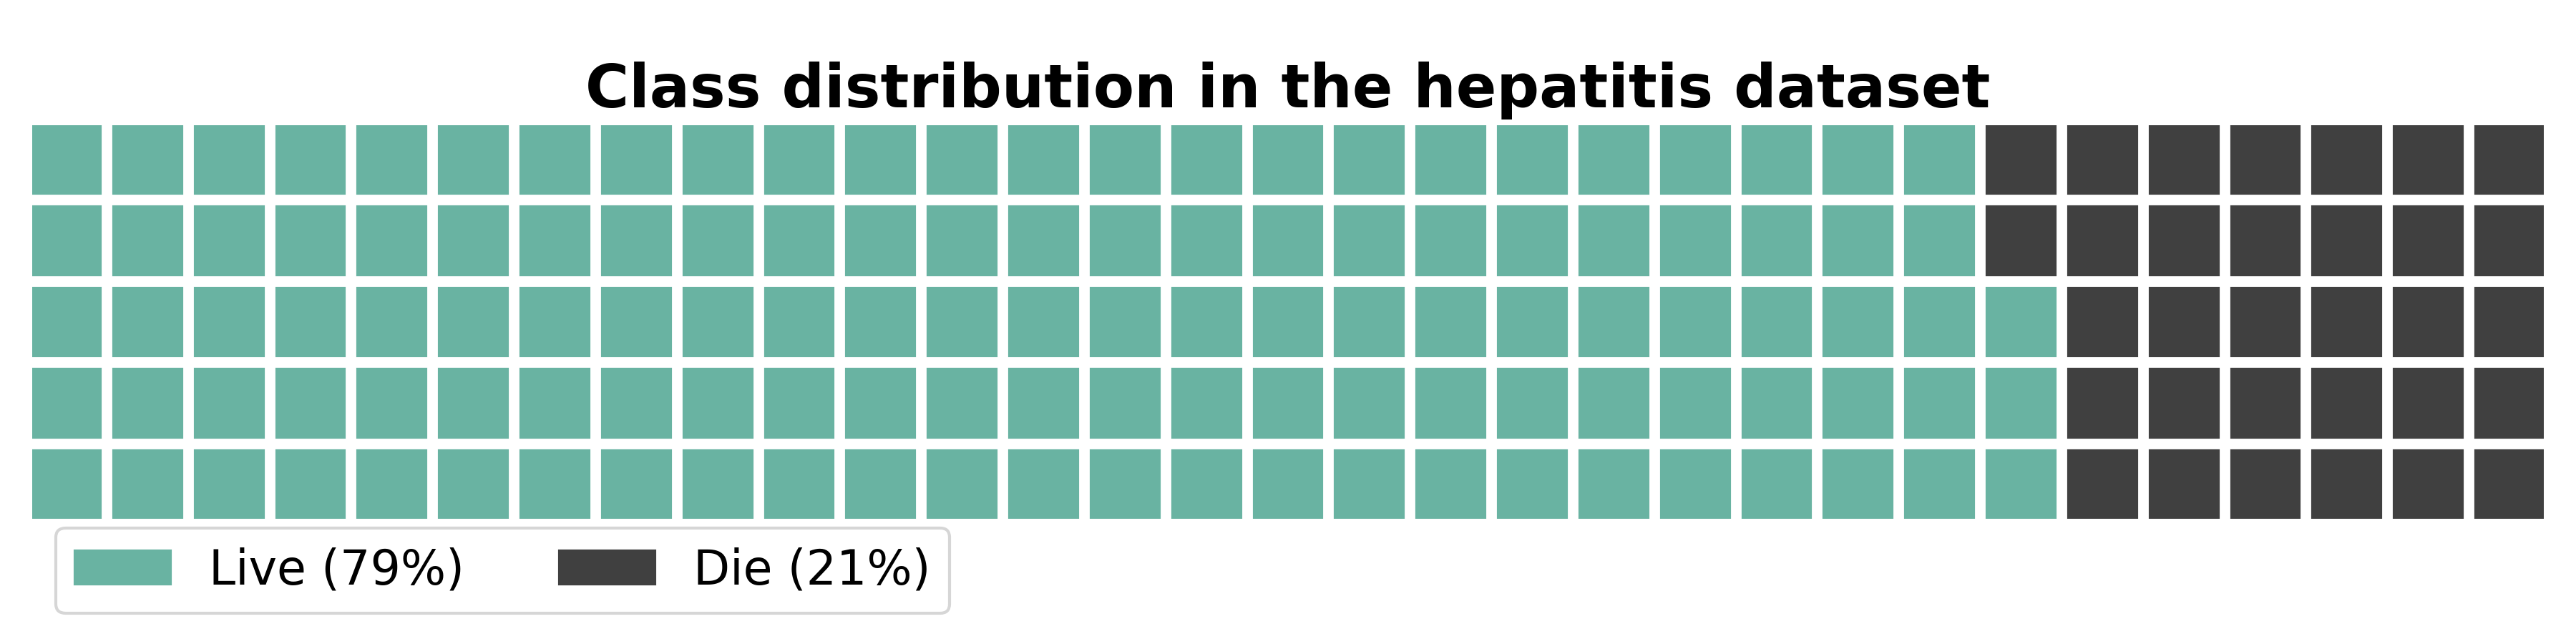
\includegraphics[width=0.9\textwidth]{figures/hepatitis-class-distribution.png}
    \caption{Class distribution of the Hepatitis dataset}
\label{fig:class-distribution-hepatitis}
\end{figure}

Furthermore, the performance metrics distribution across folds in Figure~\ref{fig:ranked-folds-knn-hepatitis} further demonstrates non-normal distribution:

\begin{figure}[!ht]
    \centering
    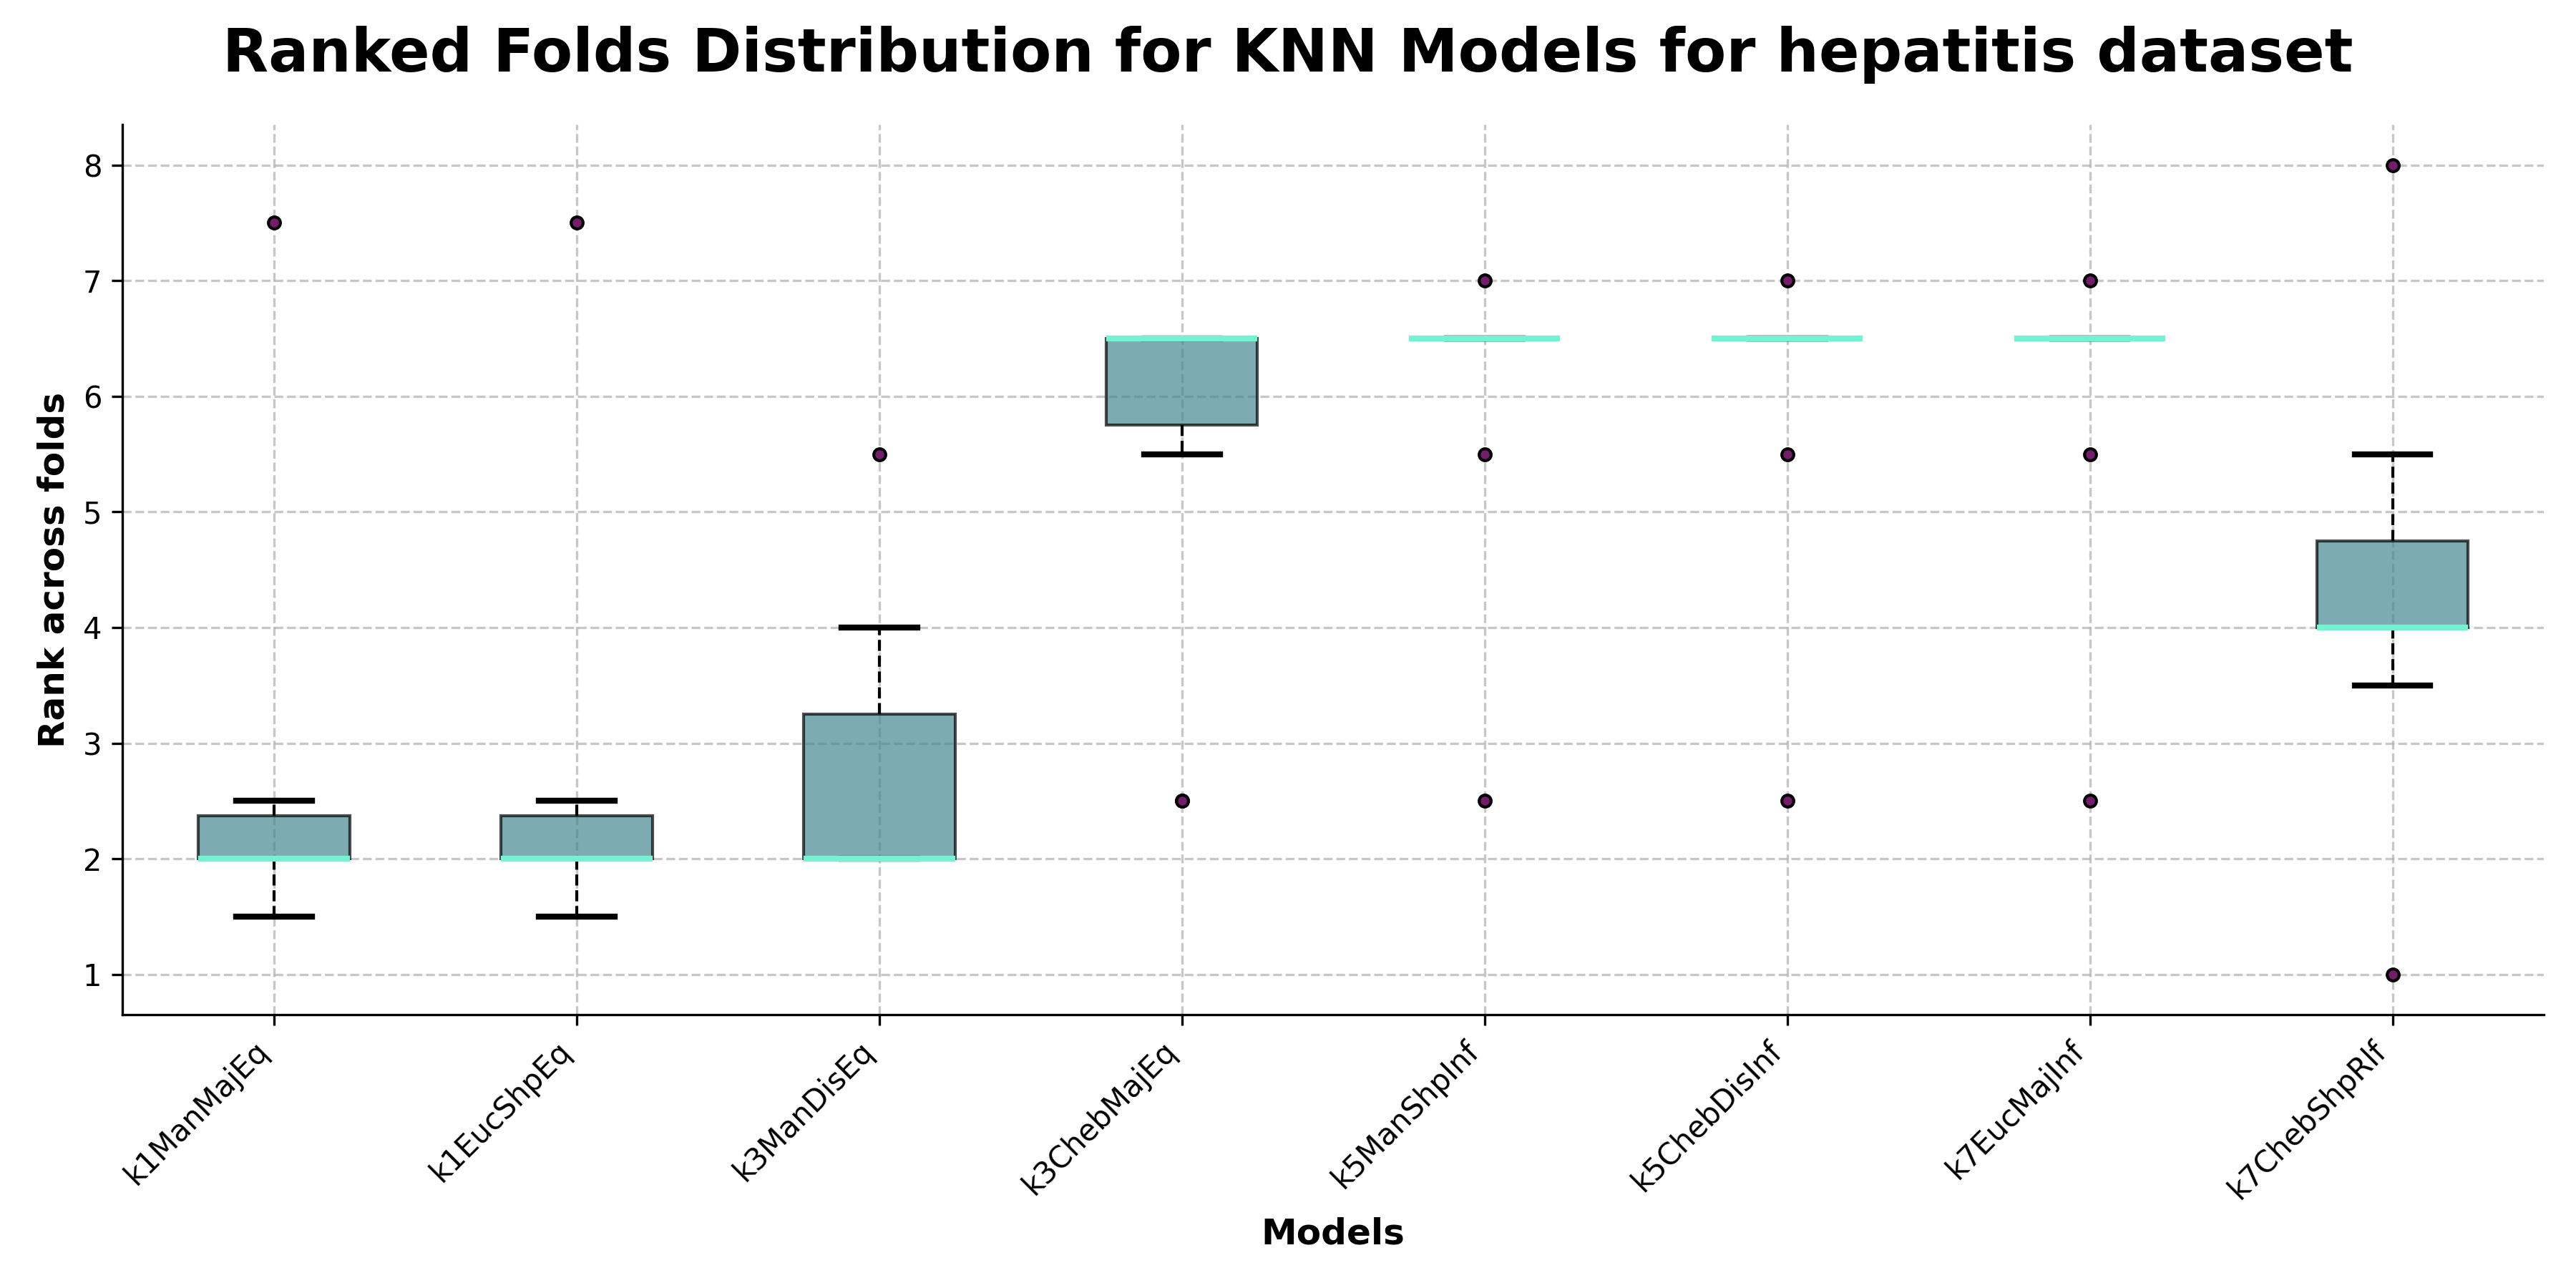
\includegraphics[width=0.9\textwidth]{figures/ranked_folds_KNN_hepatitis.png}
    \caption{Rank distributions across folds for different KNN configurations on the Hepatitis dataset}
\label{fig:ranked-folds-knn-hepatitis}
\end{figure}

These plots verify that the data does not meet the assumptions of ANOVA:

- Non-normal distribution: Several models show asymmetric distributions, where the median line is not in the middle of the box.
Also present are outliers in the data, which are represented as dots outside of the whisker lines.
- Unequal variances: Box sizes vary significantly across models, and some models have much larger spreads than others.
Additionally, the whisker lenghts vary considerably between models.

These claims hold true when analysing performance metrics distribution across folds using SVM:

\begin{figure}[!ht]
    \centering
    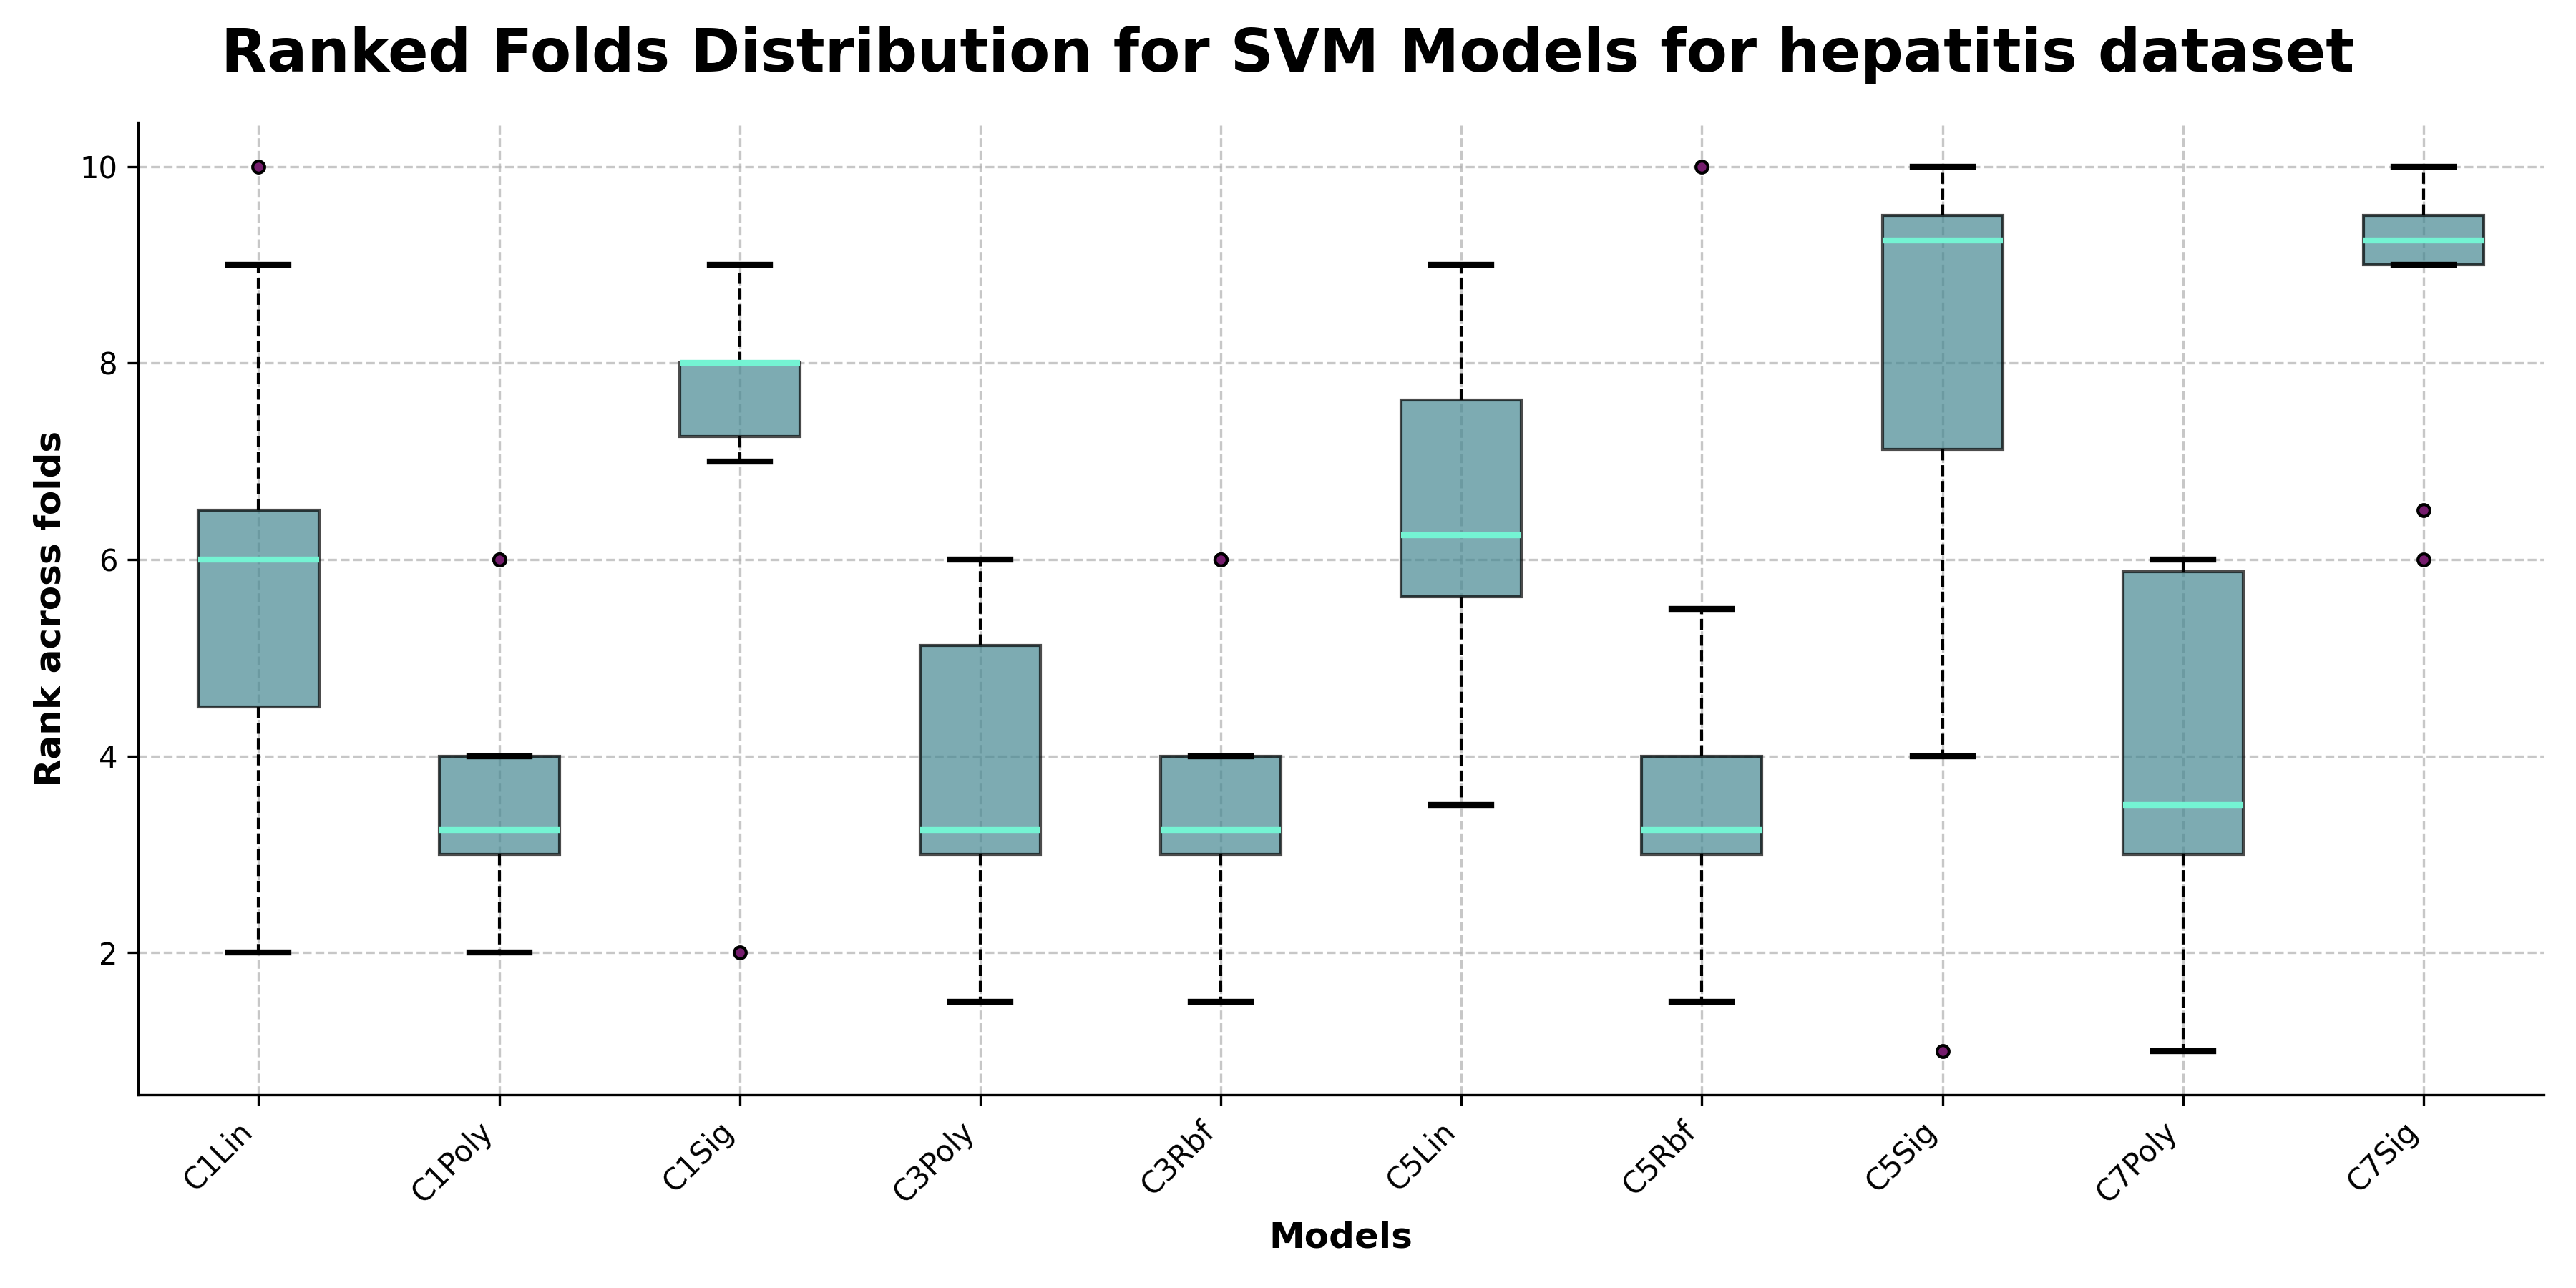
\includegraphics[width=0.9\textwidth]{figures/ranked_folds_SVM_hepatitis.png}
    \caption{Rank distributions across folds for different KNN configurations on the Hepatitis dataset}
\label{fig:ranked-folds-svm-hepatitis}
\end{figure}

Given these observations, we decided against using ANOVA for our analysis.

% TODO: Citation needed
\subsubsection*{Friedman Test}
The Friedman test is a non-parametric equivalent of the repeated-measures ANOVA. 
For each dataset, it ranks the models separately with the best model receiving a rank of 1, the second-best a rank of 2, and so on.
The average rank is used to settle any ties in the ranks [CITE].

While the Friedman test theoretically has less statistical power than ANOVA when ANOVA's assumptions are met,
it is more suitable for our analysis as it makes no assumptions about normality or equal variances.
As we demonstrated with the hepatitis dataset's class distribution and performance metrics, these assumptions do not hold in our case.

% TODO: Citation needed
\subsubsection*{Post-Hoc Tests}
The Friedman test only tells us that there is a significant difference between the models,
but it does not tell us which models are significantly different from each other.
This is why we employ the Nemenyi test as a post-hoc procedure.

The Nemenyi test compares the performance of all classifiers to each
other by checking if their average ranks differ by at least the critical difference:

\begin{equation}
    CD = q_{\alpha} \times \sqrt{\frac{k(k+1)}{6N}}
\end{equation}

where $q_{\alpha}$ is based on the Studentized range statistic, $k$ is the number of classifiers, and $N$ is the number of datasets [CITE].
If the difference in average ranks between two models exceeds this critical difference, we can conclude that their performances are significantly different.

When performing the Nemenyi test, proper handling of ties is crucial for accurate analysis.
Instead of arbitrarily assigning consecutive ranks to tied values (e.g., ranks 2 and 3), we use the
average of the ranks they would have occupied. For example, if two models tie for second place,
rather than arbitrarily assigning ranks 2 and 3, both models receive a rank of 2.5 (the average of positions 2 and 3).
This mid-rank approach ensures fair treatment of tied performances and prevents artificial rank differences that could bias the statistical analysis.

\subsection*{Test Results}
In the visualization of critical difference (CD) diagrams,the entire bar represents the critical difference value.
The half-width of the bar (CD/2) extends on either side of a model's average rank. When comparing two models,
if their CD/2 intervals do not overlap, we can conclude that there is a statistically significant difference in their performance.
This visual representation provides an intuitive way to interpret the Nemenyi test results, as any
non-overlapping bars clearly indicate significant differences between models.

\begin{figure}[h!]
    \centering
    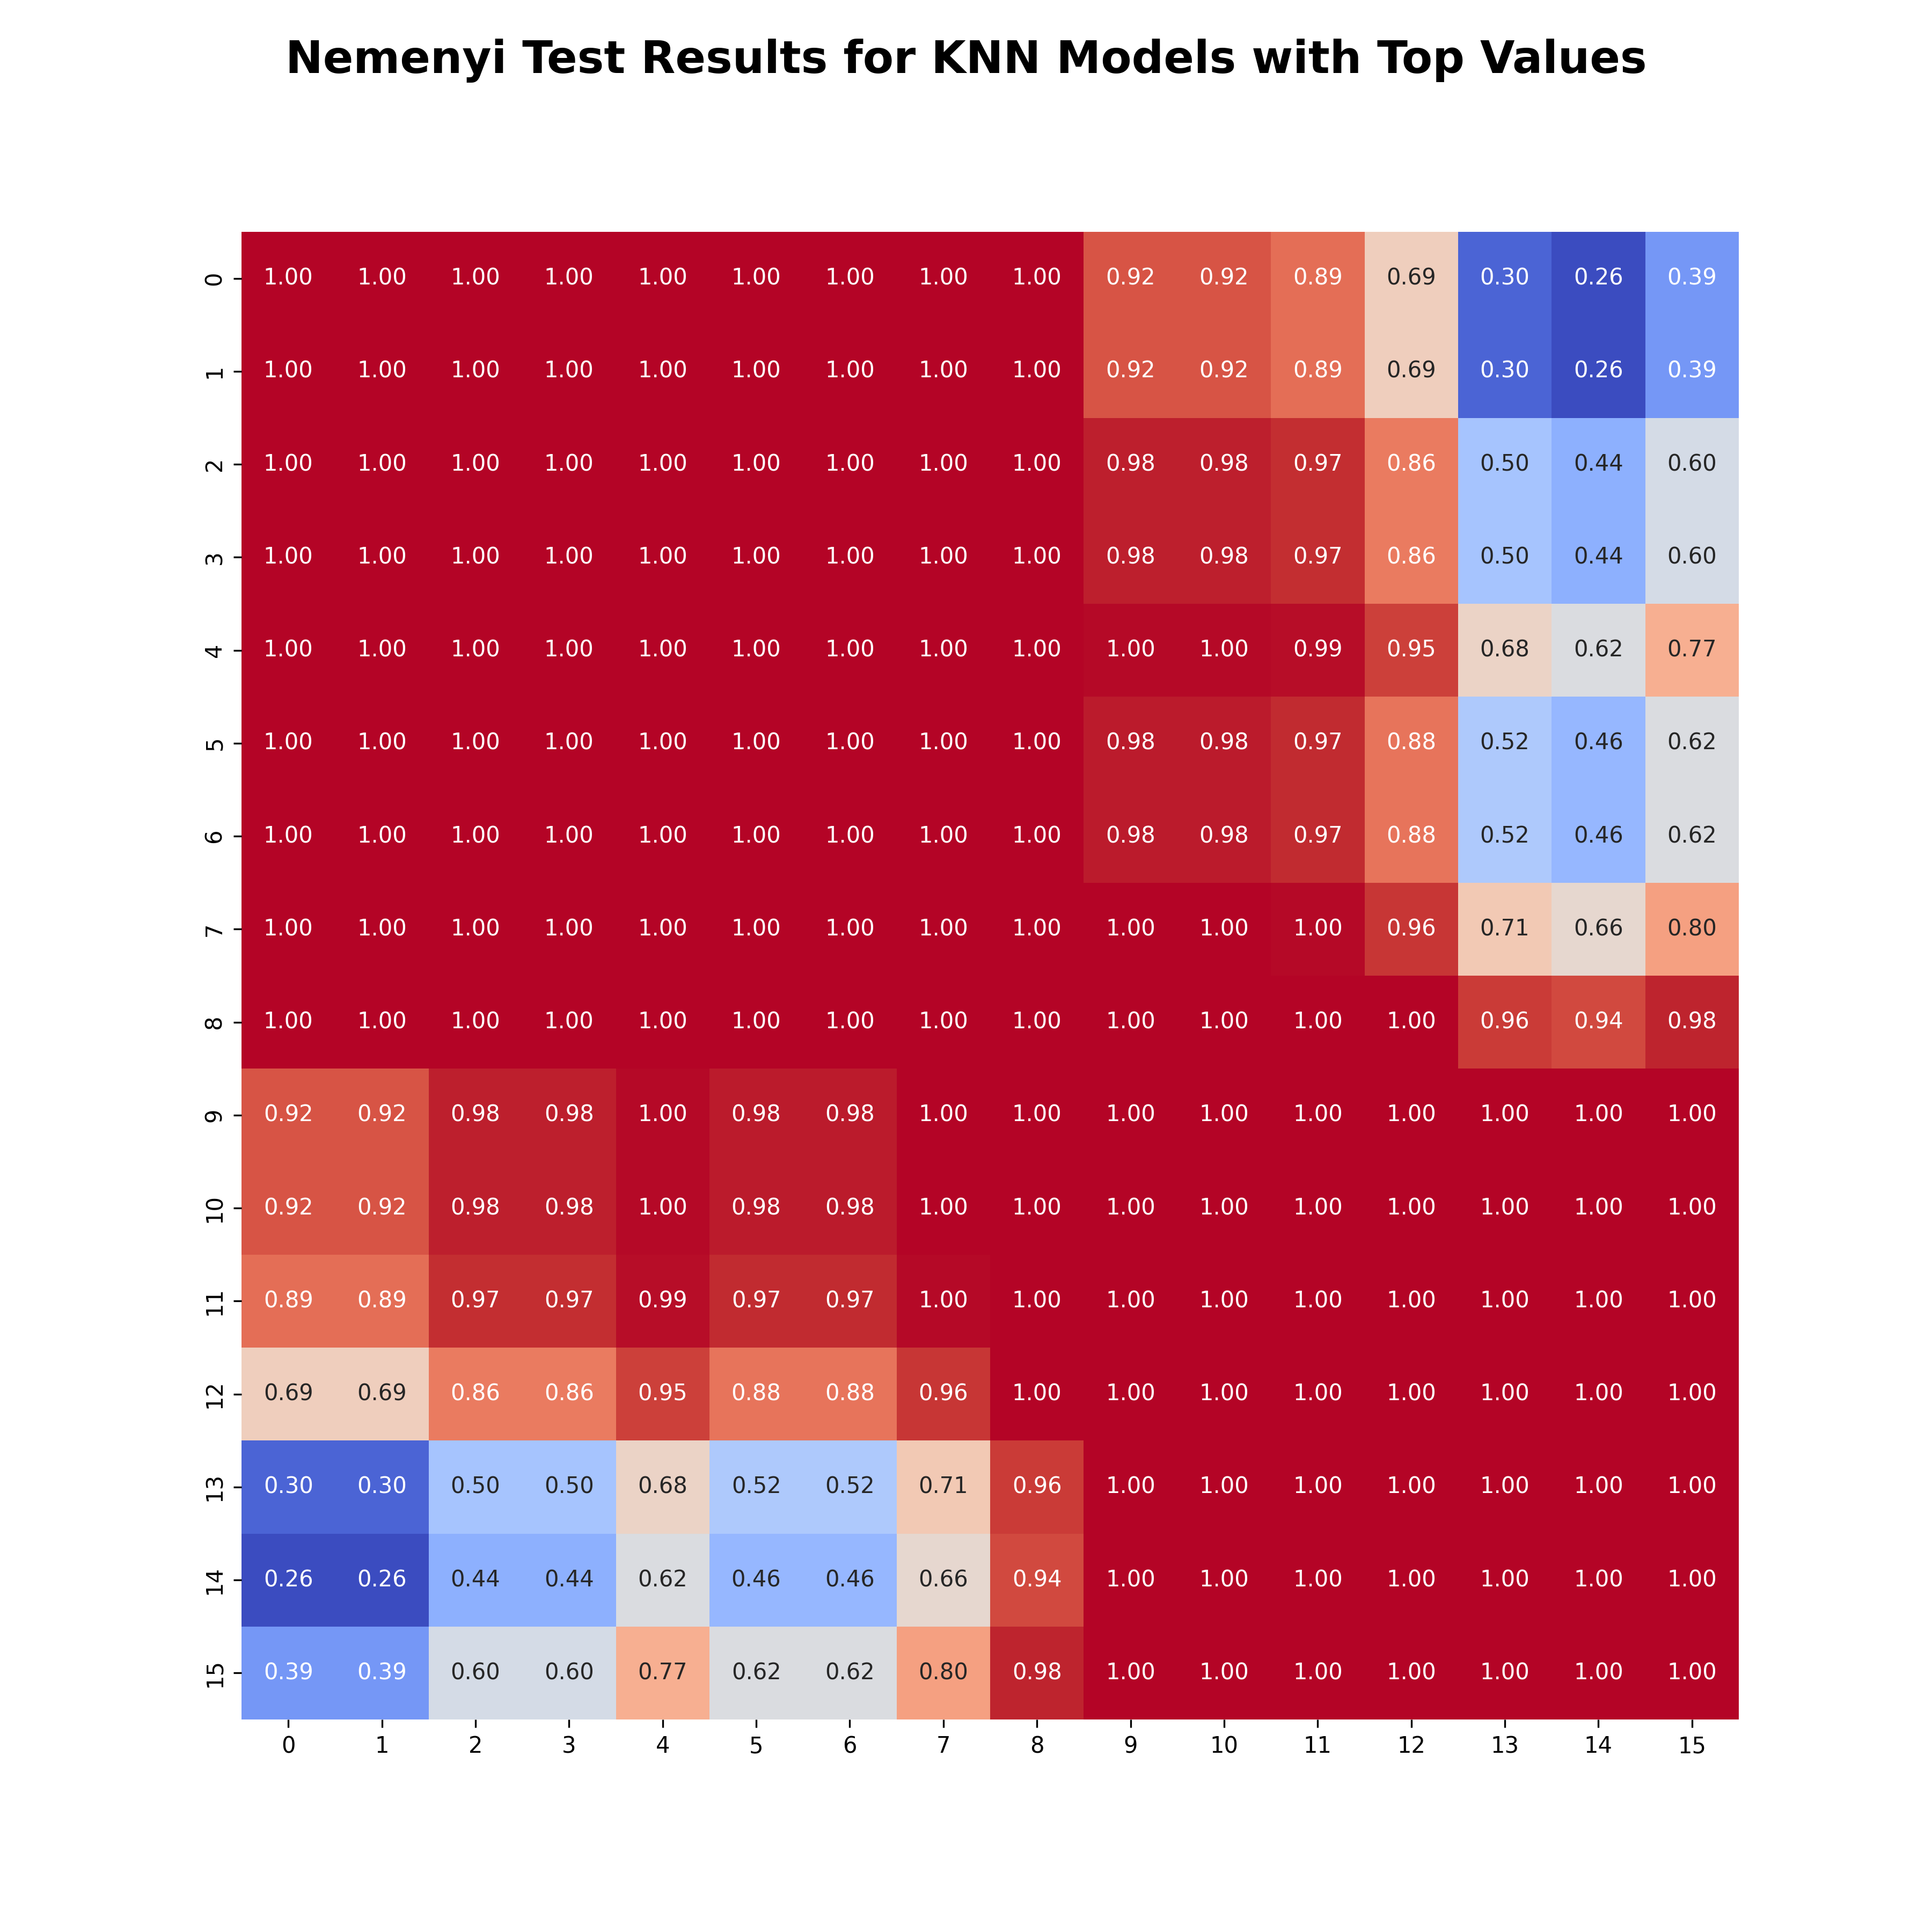
\includegraphics[width=0.9\textwidth]{figures/nemenyi_test_results_KNN_hepatitis.png}
    \caption{Pairwise comparison p-values from Nemenyi test for KNN models on the Hepatitis dataset}
\label{fig:nemenyi-knn-hepatitis}
\end{figure}

Figure~\ref{fig:nemenyi-knn-hepatitis} shows the pairwise comparison p-values from the Nemenyi test for different KNN configurations.
The heatmap uses color intensity to represent p-values, with darker red indicating higher p-values (less significant differences) and darker blue indicating lower p-values (more significant differences). Values close to 1.0 (dark red) suggest no significant difference between the corresponding models, while lower values (blue) indicate statistically significant differences in performance. We can observe clear clusters of similar-performing models, particularly in the upper-left quadrant where p-values are consistently 1.0, suggesting these configurations perform similarly.

% Plots from 'Figures' folder, and talk about what we can infer from them.

% Also need to perform empirical comparison of tests (read section 4 from the paper about this)


